\chapter{Zprovoznění jednotlivých komponent}
\label{Zprovoznění jednotlivých komponent}
Jednotlivé komponenty jsou připojeny k mikrokontroléru podle obrázku č. \ref{blokove_schema}. Displej a klávesnici stačí jen připojit, proto je nebudu v rámci této kapitoly více rozebírat.

\section{Ověření přesnosti váhy}

Před použitím samotné váhy jsem ověřil, zda její přesnost odpovídá parametrům stanoveným výrobcem z důvodu, že váha není certifikovaná. Pro ověření přesnosti byla použita váha Kern PCB-2500-2 s padesátkrát vyšší přesností, 0,01 g a váživostí 2,5 kg. Obě váhy byly před použitím kalibrovány a použity v laboratorním prostředí s teplotou 20,4 °C a vlhkostí 28,7 \%, které odpovídají požadavkům obou výrobců vah pro přesná měření. Z tabulky č. \ref{tab:vahy} je vidět, že váha G\&G-3000 měří s požadovanou přesností 0,5 g. %a spadá tak do třídy přesnosti III.


%\begin{table}
%    \centering
%    \begin{tabular}{|c|c|}
%    \hline
%         \begin{tabular}[c]{@{}c@{}} Kern PCB-2500-2 \\ (g) \end{tabular} & \begin{tabular}[c]{@{}c@{}} G\&G E3000 \\ (g) \end{tabular}\\ \hline
%         20,00 & 20,0\\ \hline
%         200,00&200,0 \\ \hline
%         400,00&400,0 \\ \hline
%         600,00 & 600,0 \\ \hline
%         800,00&800,0 \\ \hline
%         1000,00&1000,0 \\ \hline
%         1200,00&1200,0 \\ \hline
%         1400,00&1400,0 \\ \hline
%         1600,00&1600,0 \\ \hline
%         1800,00&1800,0 \\ \hline
%         2000,00&2000,0 \\ \hline
%         2200,00&2200,0 \\ \hline
%    \end{tabular}
%    \caption{Ověření přesnosti váhy G\&G E3000}
%    \label{tab:vahy}
%\end{table}

\begin{figure}[H]
    \begin{center}
        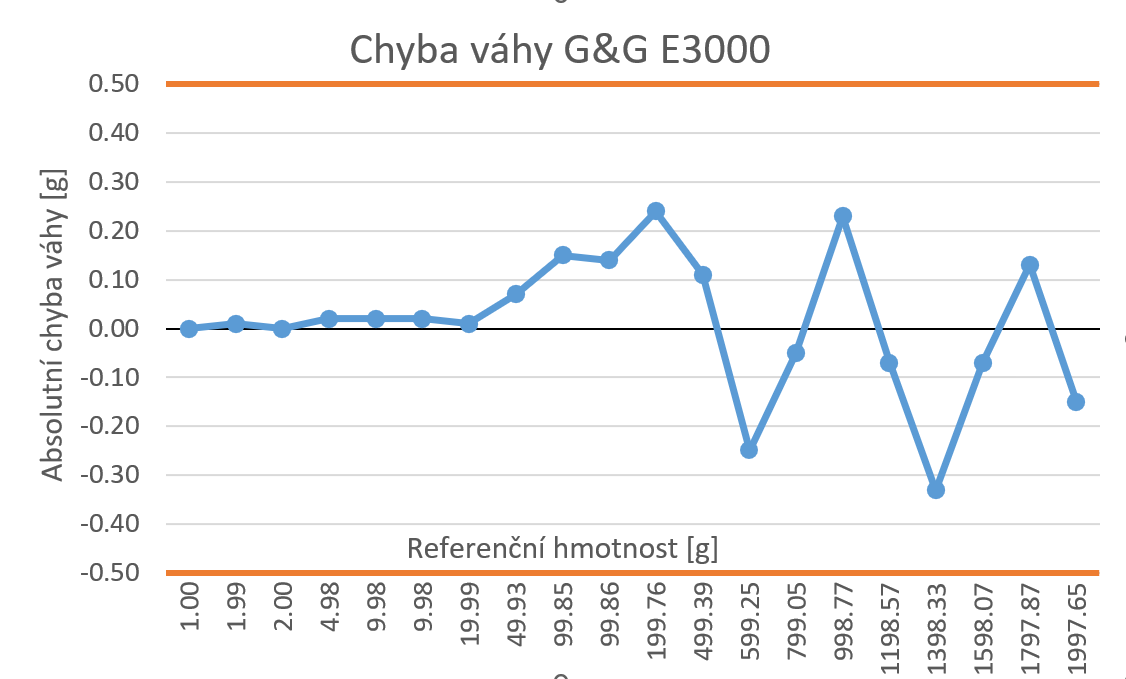
\includegraphics[scale=0.6]{obrazky/mereni.PNG}
    \end{center}
    \caption{Nalevo Kern PCB-2500-2, napravo G\&G E3000}
    \label{adapter}
\end{figure}

\begin{figure}[H]
    \begin{center}
        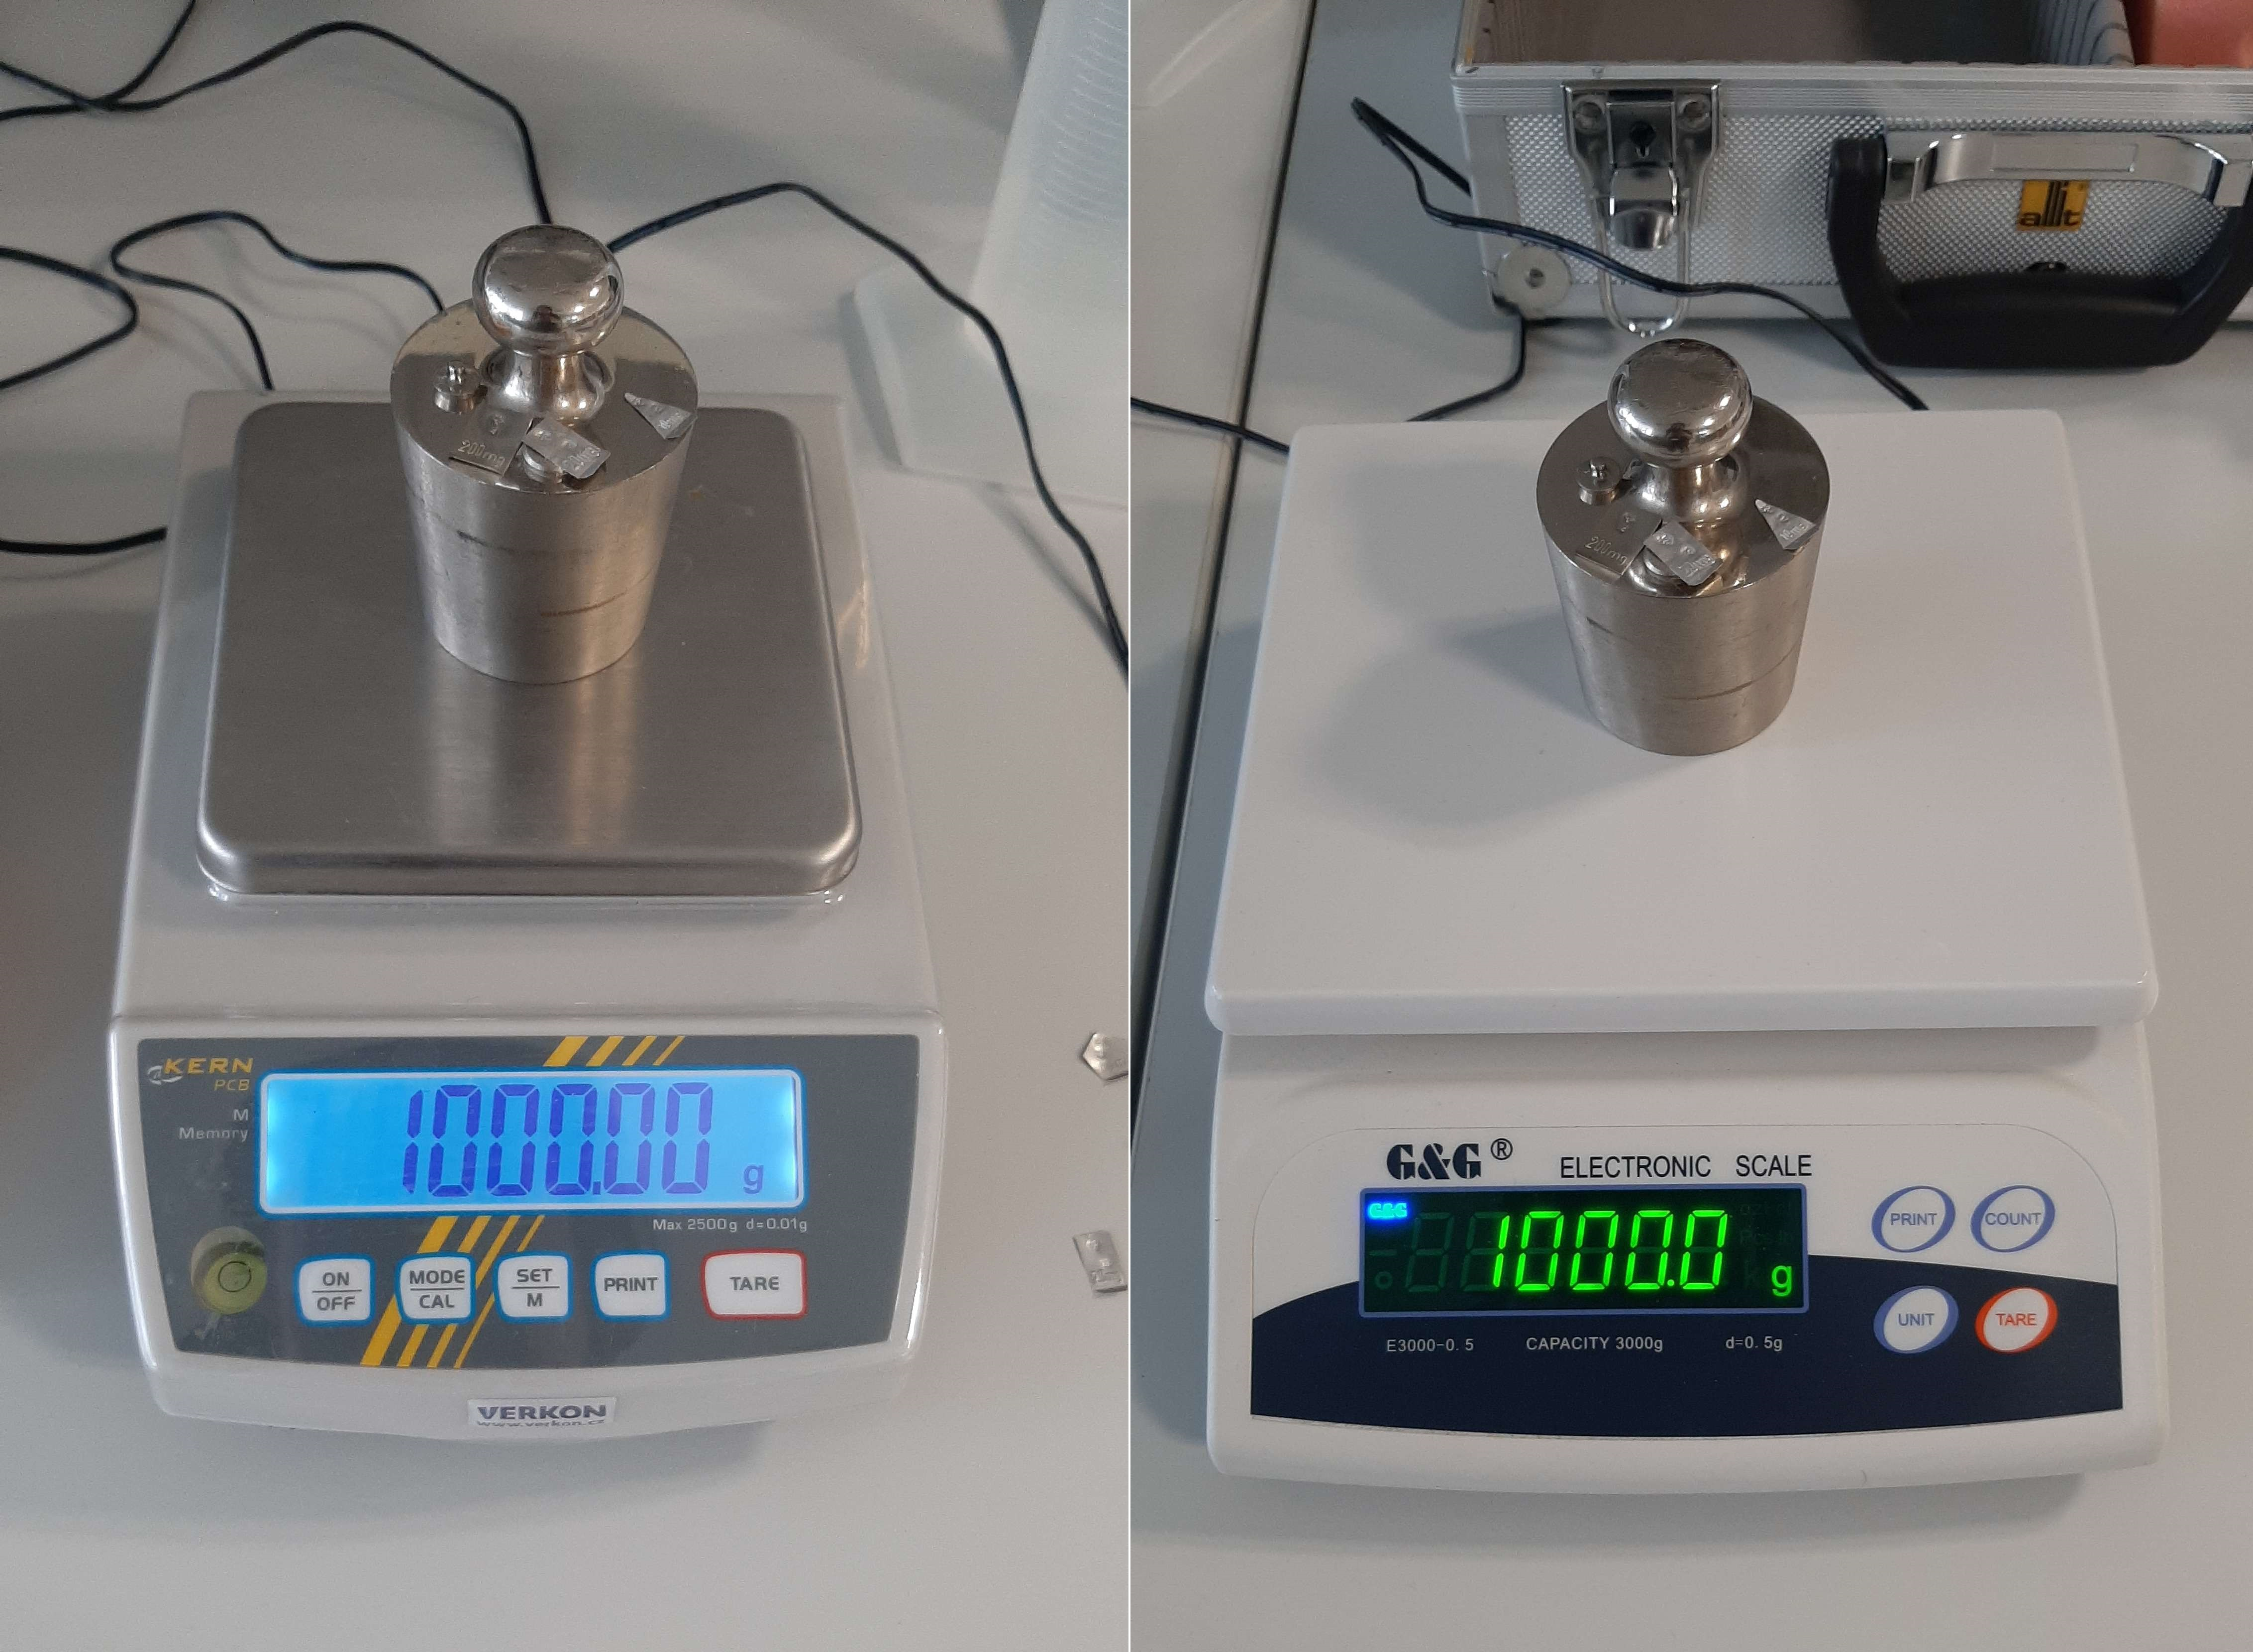
\includegraphics[scale=0.1]{obrazky/vahy.jpg}
    \end{center}
    \caption{Nalevo Kern PCB-2500-2, napravo G\&G E3000}
    \label{adapter}
\end{figure}

\section{Zprovoznění váhy}

Komunikační rozhraní váhy je RS-232, který nejsme schopni připojit na mikrokontrolér z důvodu absence totožného rozhraní. V takovém případě použijeme adaptér z RS-232 na USB. Použitý adaptér je ADS-50 USB - serial, který je součástí balení váhy. (obrázek č.\ref{adapter})

\begin{figure}[!h]
    \begin{center}
        \includegraphics[scale=0.04]{obrazky/ADS-50 USB - serial adapter.png}
    \end{center}
    \caption{Adaptér USB - serial AXAGO ADS-50}
    \label{adapter}
\end{figure}

Propojení kabelu ADS-50 s váhou není možné z důvodu, že kabel není křížený, jinak zvaný "null modem" kabel. To znamená, že vysílací piny(Tx) jsou navzájem propojené a to samé přijímací piny(Rx). Aby komunikace mohla fungovat je nutné propojit Tx s Rx. Tato podmínka komunikace je zmíněná v dokumentaci váhy[x]. Výrobce váhy z tohoto důvodu k balení přidal kříženou redukci DB9(samice) - DB9(samice), která slouží současně k monitorování stavu jednotlivých pinů díky přídavným konektorům pro připojení např. osciloskopu. Dále výrobce přidal redukci DB9(samec) - DB9(samec) pro propojení křížené redukce s váhou(samice). Zapojení je možné vidět na obrázku č.\ref{propojení váhy v1}. Toto zapojení není praktické pokud nechceme diagnostikovat komunikaci, proto je možností koupit přímo křížený kabel nebo kříženou redukci, která vychází 5x levněji. Na obrázku č.\ref{propojení váhy v2} je výsledné řešení propojení váhy s mikrokontrolerem pomocí křížené redukce DB9(samec) - DB9(samice).

\begin{figure}[!h]
    \begin{center}
        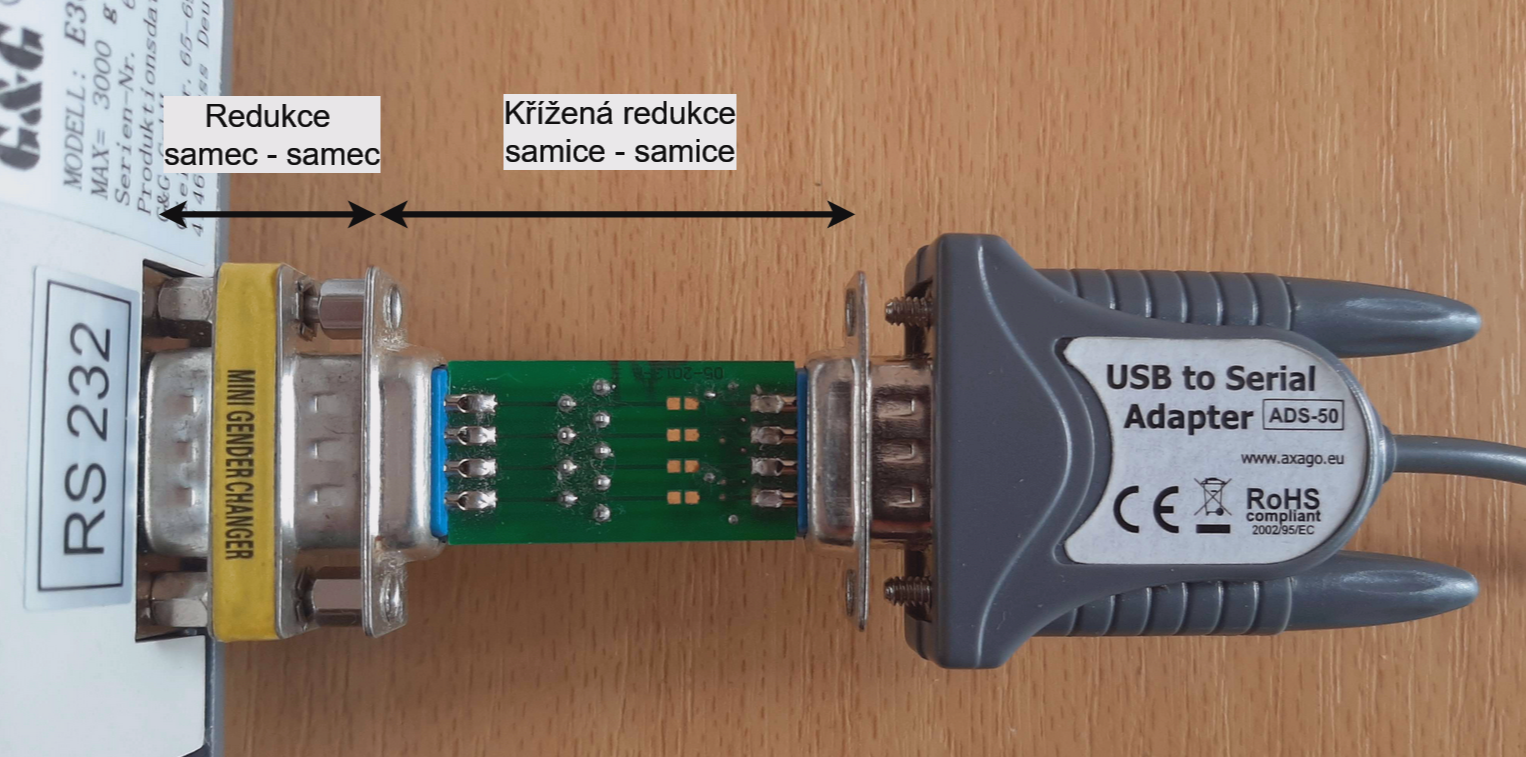
\includegraphics[scale=0.27]{obrazky/zapojeni_vahy_v1 - popis.png}
    \end{center}
    \caption{Propojení váhy s mikrokontrolerem pomocí komponent dodané výrobcem váhy}
    \label{propojení váhy v1}
\end{figure}

\begin{figure}[!h]
    \begin{center}
        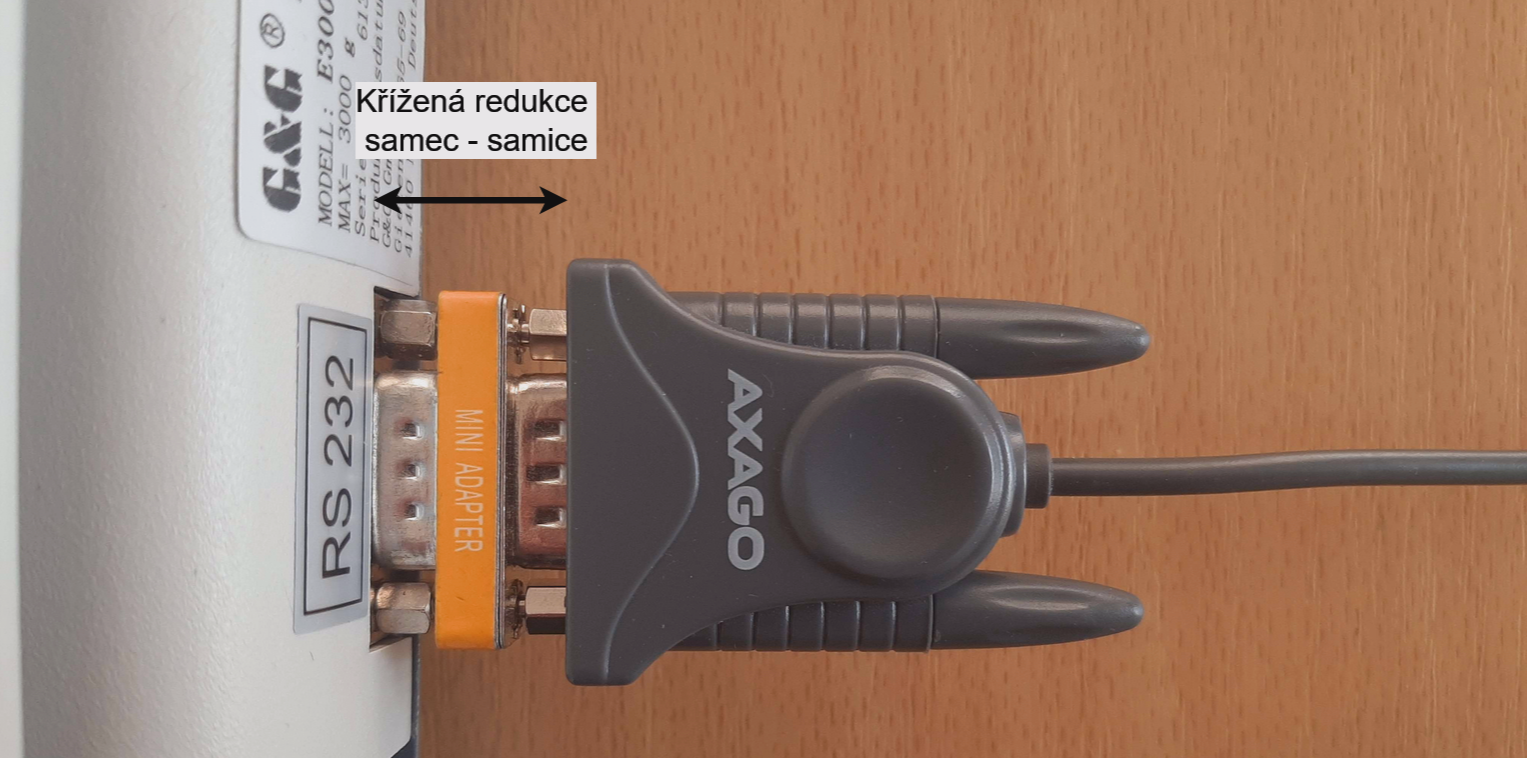
\includegraphics[scale=0.27]{obrazky/zapojeni_vahy_v2 - popis.png}
    \end{center}
    \caption{Výsledné propojení váhy s mikrokontrolerem}
    \label{propojení váhy v2}
\end{figure}

Dalším krokem je nastavení parametrů sériové komunikace podle manuálu váhy\cite{vaha_datasheed}. Komunikace byla testována pomocí osciloskopu s funkcí čtení UART protokolu a windows nástroje PuTTY, který přijímal/odesílal data po sériové lince. 
Na obrázku č. \ref{putty} je nastavení parametrů v PuTTY a na obrázku č.\ref{puttyyyy} je vidět, že váha nám na výstup konzole PuTTY posílá aktuální naměřená data.


\begin{figure}[!h]
    \begin{center}
        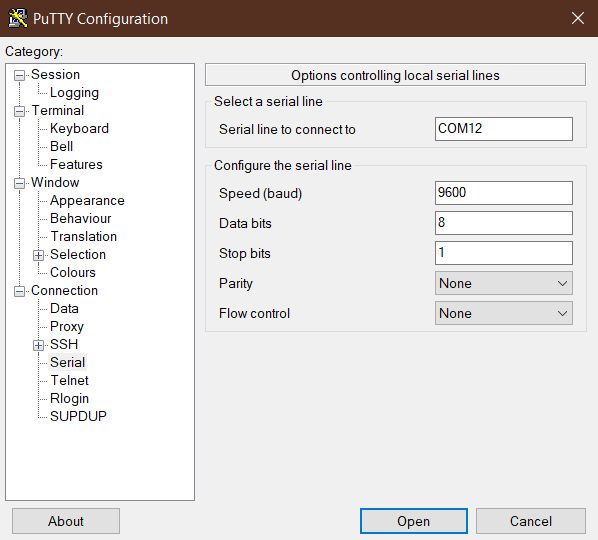
\includegraphics[scale=0.8]{obrazky/nastaveni putty.png}
    \end{center}
    \caption{Nastavení parametrů komunikace v PuTTY}
    \label{putty}
\end{figure}

\begin{figure}[!h]
    \begin{center}
        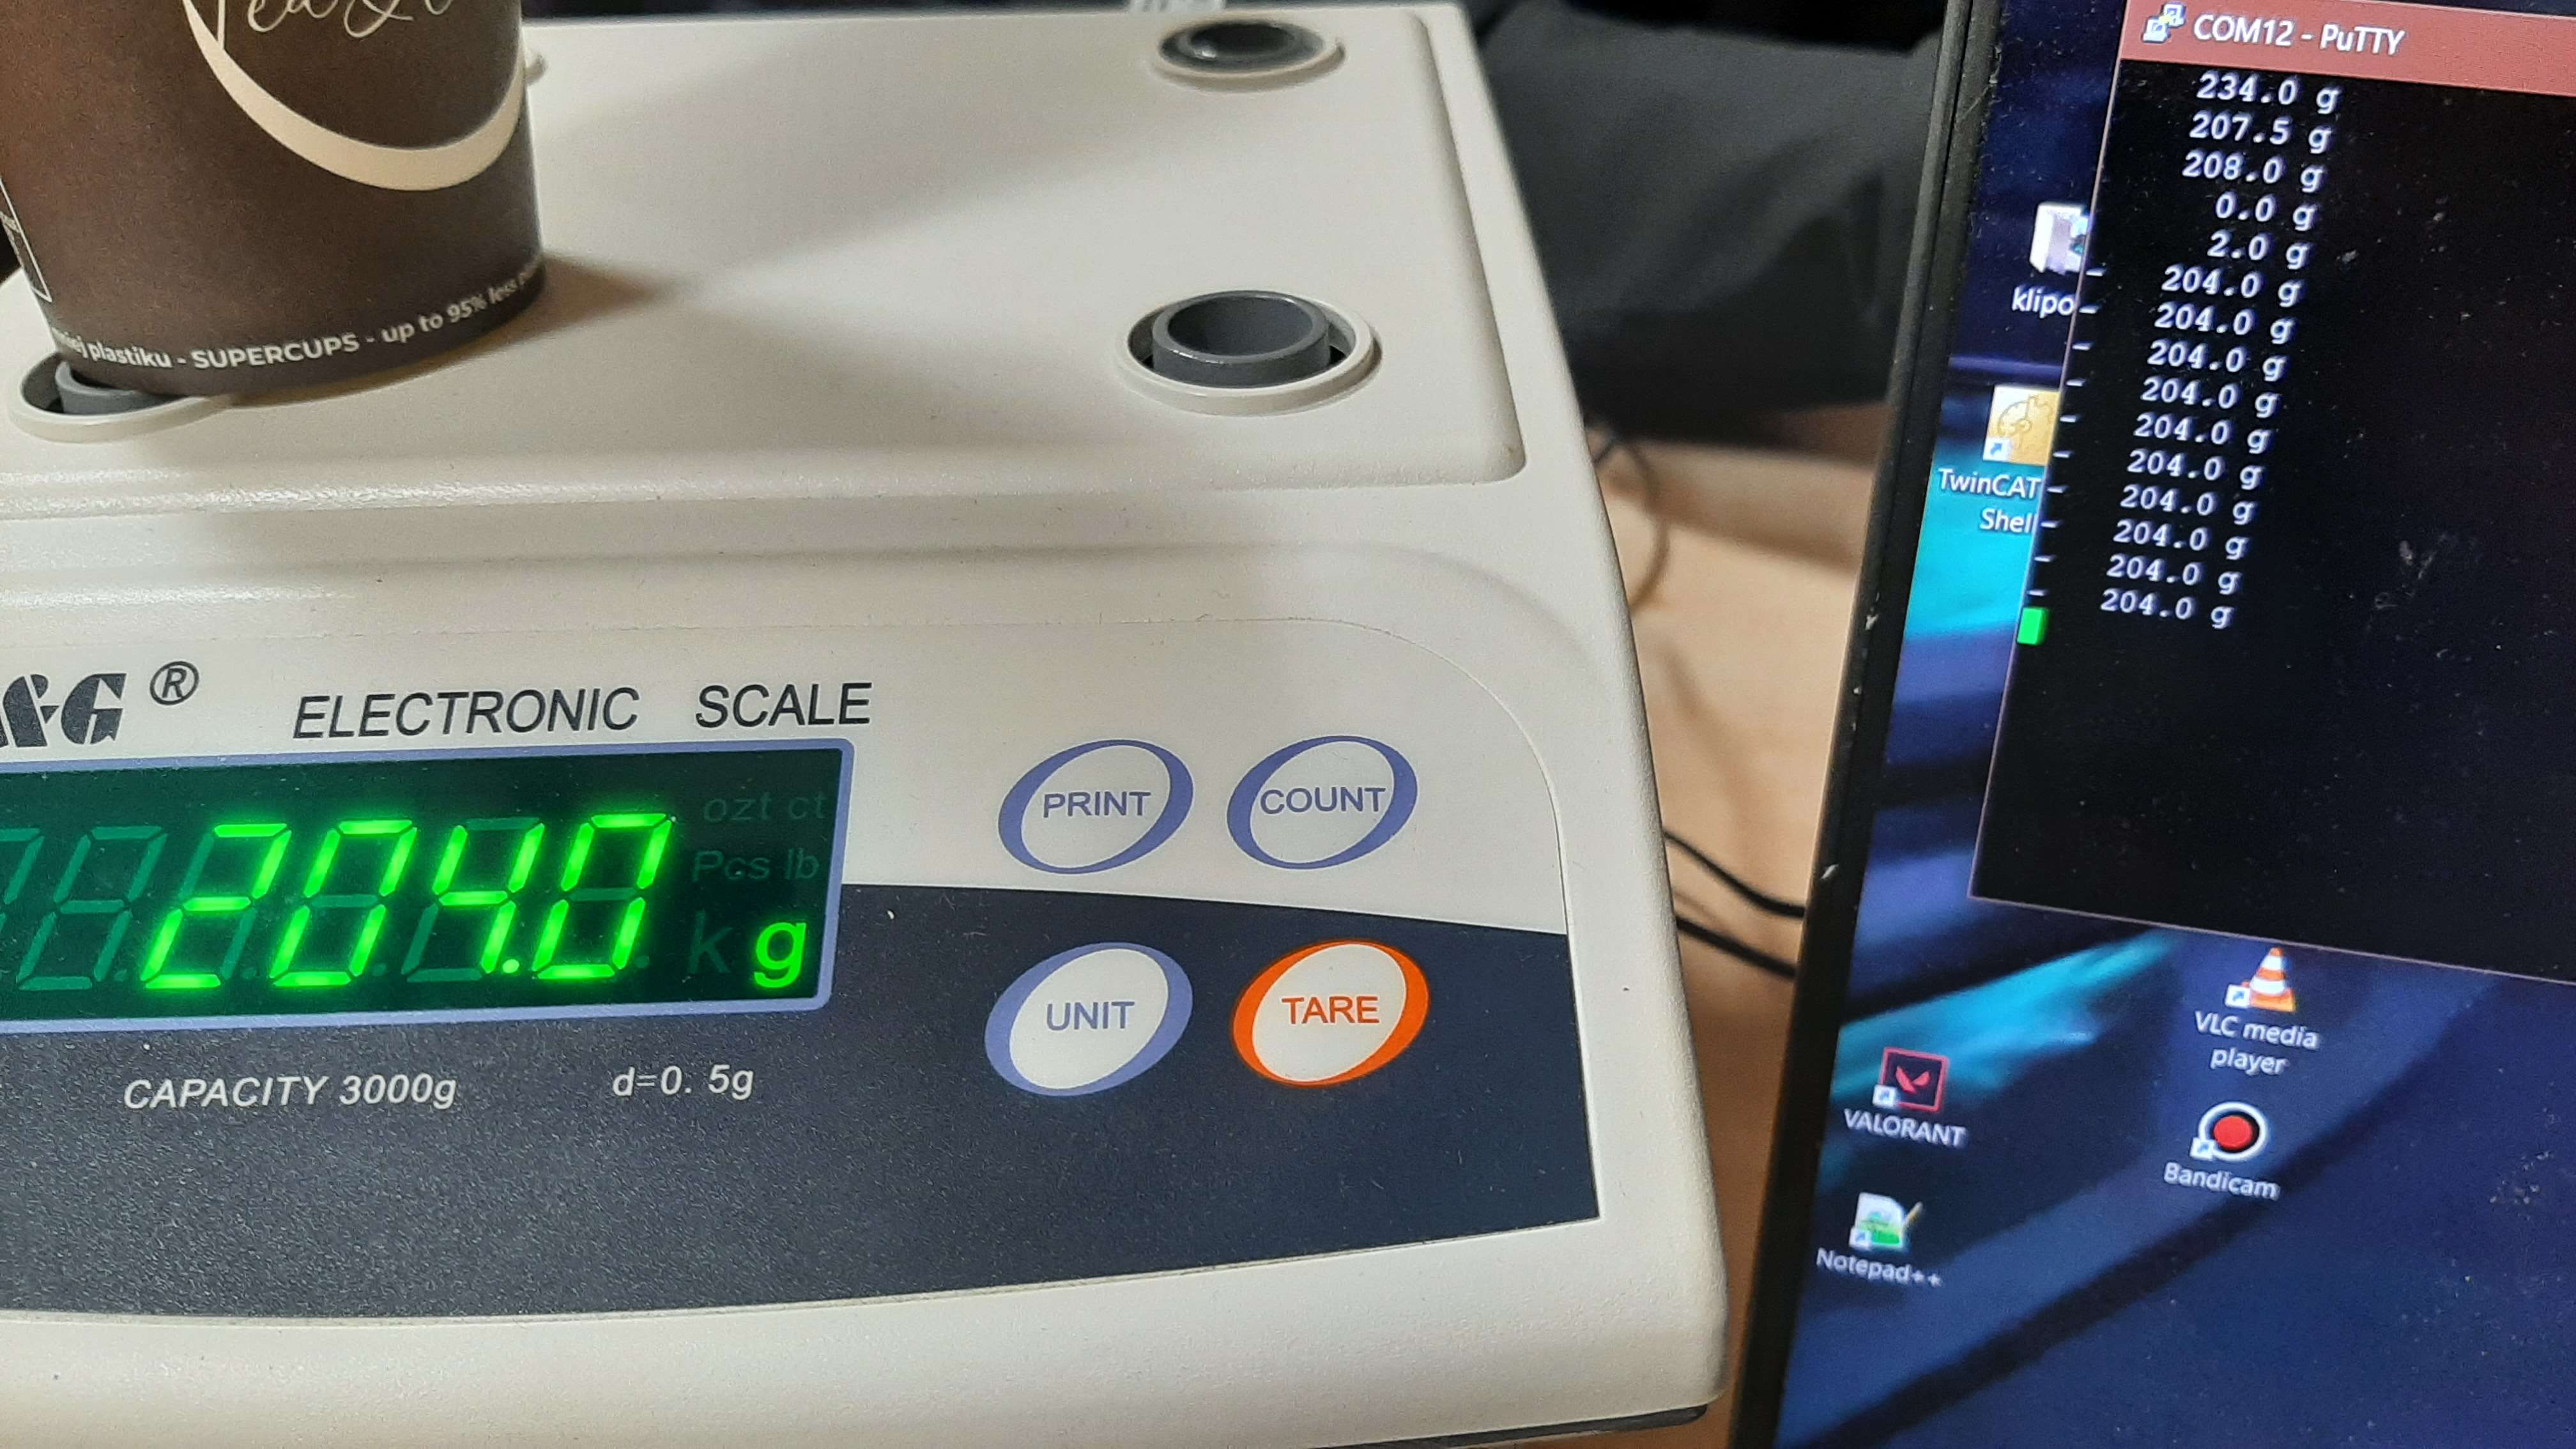
\includegraphics[scale=0.09]{obrazky/Testování komunikace pomocí PuTTY.jpg}
    \end{center}
    \caption{Čtení sériové komunikace váhy pomocí PuTTY}
    \label{puttyyyy}
\end{figure}

Na obrázku č.\ref{osc} byl datový výstup váhy testován pomocí osciloskopu. Parametry na osciloskopu byly nastaveny obdobně jak na obrázku č.\ref{putty}

\begin{figure}[!h]
    \begin{center}
        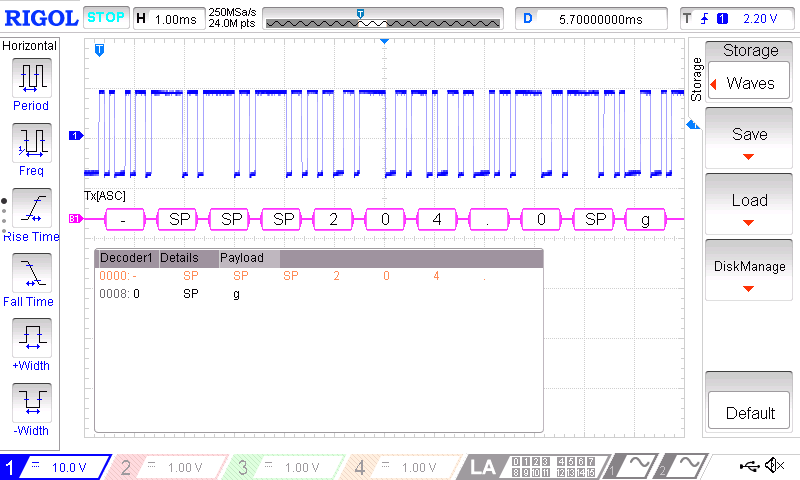
\includegraphics[scale=0.5]{obrazky/DS1Z_QuickPrint6.png}
    \end{center}
    \caption{Odchycení zprávy "-204.0 g" pomocí osciloskopu}
    \label{osc}
\end{figure}

\section{Zprovoznění čtečky čárového kódu}
\label{zprovozeni_ctecky}
Čtečka čárového kódu ve výchozím nastavení se chová jako klávesnice(HID KBW), aby bylo možné číst sériovou komunikaci je nutné naskenovat QR kód z manuálu\cite{scaner}, který přepíná výstup čtečky z HID KBW na virtuální sériový USB port(USB VCom).\\\\
%Čtečku čárového kódu lze připojit pomocí UART nebo USB rozhraní. 

\section{Zprovoznění dotykového displeje}
Vybraný dotykový displej xxx, má rozlišení 1024x600 px s poměrem stran 128:75, což přibližně odpovídá poměru 17:10. Raspberry Pi OS vybírá rozlišení podle seznamu podporovaných rozlišení CEA (Consumer Electronics Association) a DMT (Display Monitor Timings), které jsou standardní a široce kompatibilní s většinou monitorů a televizí. Rozlišení vybraného displeje nespadá do žádné zmíněné kategorie a je nutné jej nastavit ručně prostřednictvím systémového souboru 'config.txt' .[z1][z2] Pokud by rozlišení displeje se neshodovalo s rozlišením obrazovky, tak by se obraz musel škálovat (upraven tak, aby se vešel na fyzický rozměr displeje, což znamená jeho zvětšení nebo zmenšení), což by vedlo ke snížení kvality obrazu, dále pokud by rozlišení obrazovky překročilo rozlišení displeje, tak by došlo k většímu vytížení GPU.

\subsection{Nastavení rozlišení obrazovky pomocí utility Xrandr}
%Použijem příkaz "cvt" (Coordinated Video Timing), který pro zvolené rozlišení vypíše informaci, jako je obnovovací frekvence, horizontální frekvence synchronizace (hsync) a pixel clock (pclk). Tyto informace jsou nutné pro nastavení nového rozlišení pomocí Xrandr.

Pro nastavení nového rozlišení využíváme příkaz "cvt" (Coordinated Video Timing), který poskytuje podrobné informace o zvoleném rozlišení, včetně obnovovací frekvence, horizontální frekvence synchronizace (hsync) a pixel clock (pclk). Tyto údaje jsou nezbytné pro konfiguraci nového rozlišení pomocí nástroje Xrandr.
\\
\\
Příklad použití příkazu cvt:
\\
\$ cvt 1024 600
\\
\# 1024x600 59.85 Hz (CVT) hsync: 37.35 kHz; pclk: 49.00 MHzxa
Modeline "1024x600\_60.00"   49.00  1024 1072 1168 1312  600 603 613 624 -hsync +vsync
\\
\\
Následně vytvoříme nový režim pomocí Xrandr:
\\
\$xrandr --newmode  "1024x600\_60.00"   49.00  1024 1072 1168 1312  600 603 613 624 -hsync +vsync
\\
\\
Nově vytvořený režim přidáme k požadovanému video výstupu (HDMI-1):
\\
\$xrandr --addmode HDMI-1 "1024x600\_60.00"
\\
\\
Nyní změníme rozlišení obrazovky pomocí:
\\
\$xrandr --output HDMI-1 --mode "1024x600\_60.00"
\\
\\
%Toto nastavení se neukládá a pokud chceme mít nově nastavené rozlišení i po opětovném spuštění raspberry pi je nutné jej uložit do souboru, který se spouští současně se systémem jako např. /etc/X11/xorg.conf.d/10-monitor.conf

Toto nastavení není trvalé a aby zvolené rozlišení zůstalo zachováno i po opětovném spuštění Raspberry Pi, je třeba jej uložit do konfiguračního souboru, například /etc/X11/xorg.conf.d/10-monitor.conf.




%Nastavení rozlišení obrazovky pomocí systé

%V případě zvětšení(upscaling) by obraz ztrácel na přesnosti a byl by rozmazaný, zatím co při zmenšení(downscaling) by obraz ztrácel na detailech

%z1: raspbery dokumentace - co je v zadání BP
%z2: https://elinux.org/RPiconfig#Camera